% ------------------------------------------
% Datenbanksysteme
% Sommersemester 2017
% Projektdokumentation
%
% Andreas Timmermann
% Alena Dudarenok
% Julian Meyer
% Ailis Oßwald
% ------------------------------------------
\documentclass[a4paper ,8pt,x11names]{article}
\usepackage[utf8]{inputenc}
\usepackage{pdflscape}
\usepackage{tikz}
\usetikzlibrary{er}
\usetikzlibrary{positioning}
\usepackage{caption, booktabs}
\usepackage[autostyle=true,german=quotes]{csquotes}
\usepackage{amsmath}

\tikzset{multi attribute/.style={attribute,double distance=1.5pt}} 
\tikzset{derived attribute/.style={attribute ,dashed}} 
\tikzset{total/.style={double distance=2.5pt}}
\tikzset{total2/.style={double distance=15.0pt}}
\tikzset{every entity/.style={draw=orange, fill=orange!20}}
\tikzset{every attribute/.style={draw=MediumPurple1, fill=MediumPurple1!20}} \tikzset{every relationship/.style={draw=Chartreuse2, fill=Chartreuse2!20}} \newcommand{\key}[1]{\underline{#1}}

\begin{document}
% ------------------------------------------
% Startseite
% ------------------------------------------
\begin{center}
\Huge{\textbf{Projektdokumentation}}\\
\Large{\textbf{Datenbanksysteme 2017}}\\
\normalsize
\vspace{4cm}
\underline{\textbf{Autoren}}\\
Timmermann, Andreas\\
Dudarenok, Alena\\
Meyer, Julian\\
O\ss wald, Ailis\\
\normalsize
\end{center}
\newpage
% ------------------------------------------
% Projektziel
% ------------------------------------------
\begin{flushleft}
\vspace{0.25cm}
\textbf{1.1 Projektziel}
\vspace{0.25cm}\\
Es soll eine Web-Anwendung erstellen werden mit der der Datensatz "american-election" visualisiert werden kann. Des weiteren soll es möglich sein Anfragen an eine Datenbank zu stellen, um bestimme Informationen und Zusammenhänge zu erhalten und deren Entwicklung über die Zeit.\\
Zum Beispiel werden Abfragen für Häufigkeiten von Hashtags in Tweets möglich sein, aber auch die visuelle Darstellung von häufig genutzten Hashtags und die Entwicklung über einen bestimmten Zeitraum.\\ 
Hauptsächlich geht es um die Analyse der Hashtags und deren Nutzung, weniger um den Inhalt der Tweets.
% ------------------------------------------
% Das Team
% ------------------------------------------
\vspace{0.25cm}\\
\textbf{1.2 Das Team}
\vspace{0.25cm}\\
Andreas Timmermann, 4. Semester, Informatik Monobachelor\\
Alena Dudarenok, 4. Semester, KomboInformatik (Kernfach Informatik)\\
Julian Meyer, 5. Semester, Informatik Monobachelor\\
Ailis Oßwald, 4. Semester, Informatik Monobachelor
% ------------------------------------------
% Explorative Datenanalyse
% ------------------------------------------
\vspace{0.25cm}\\
\textbf{2. Explorative Datenanalyse}
\vspace{0.25cm}\\
Der Datensatz "american-election" kann auch schon als Datenbank angesehen werden. Dabei gibt es eine Entität, die die ganze Tabelle mit 11 Spalten als deren Attribute umfässt.\\
%Es folgt eine Auflistung aller Attribute dieser Tabelle:\\

\begin{table}[!htb] 
 \begin{tabular}{|c|p{8cm}|}\hline
   \textbf{Attribute} & \textbf{Beschreibung} \\ \hline \hline
   handle & gibt an ob der Tweet auf Hillarys oder Trumps Profil steht \\ \hline
   text & Inhalt des Tweets mit Hashtags \\ \hline
   is\_retweet & enthält ein Boolean, der angibt, ob der Tweet ein retweet ist \\ \hline
   original\_author & falls is\_retweet == true, wird hier der Twittername des Originalautors angegeben \\ \hline
   time & Zeitstempel des Tweets \\ \hline
   in\_reply\_to\_screen\_name & Antwort auf Nutzername \\ \hline
   is\_quote\_status & ein Boolean, der angibt, ob das ein Retweet mit zusätzlichem Text ist \\ \hline
   retweet\_count & wie oft der Tweet retweetet wurde \\ \hline
   favourite\_count & Anzahl der "Likes" \\ \hline
   source\_url & von was für einem Gerät der Tweet gesendet wurde \\ \hline
   truncated & ein Boolean, der angibt, ob der Tweet gekürzt ist \\ \hline
 \end{tabular}
\end{table}
\end{flushleft}

\newpage
% ------------------------------------------
% ER-Diagramm
% ------------------------------------------
\large{\textbf{\underline{3. ER-Diagramm (Chen-Notation)}}}\\

\begin{center}
  \resizebox{\textwidth}{!}{
\begin{tikzpicture}[node distance=10em]
\node[relationship] (KommtVorIn) {KommtVorIn}; 
\node[entity] (Hashtag) [left=3.0cm of KommtVorIn] {Hashtag} edge[total] node [above left=0.25cm]{m} (KommtVorIn); 
\node[attribute] (Name) [above left=2.5cm of Hashtag] {\key{Name}} edge (Hashtag); 
\node[attribute] (HaeufigkeitGesamt) [above=2.5cm of Hashtag] {HaeufigkeitGesamt} edge (Hashtag); 
\node[entity] (Tweet) [right=4.0cm of KommtVorIn] {Tweet} edge node [above right=0.25cm]{n} (KommtVorIn); 
\node[attribute] (AnzRetweets) [above left=2.5cm of Tweet] {AnzRetweets} edge (Tweet); 
\node[attribute] (AnzLikes) [above=2.5cm of Tweet] {AnzLikes} edge (Tweet); 
\node[attribute] (Handle) [above right=2.5cm of Tweet] {Handle} edge (Tweet); 
\node[attribute] (TweetID) [right of=Tweet] {\key{TweetID}} edge (Tweet); 
\node[attribute] (OriginalAutor) [below right of=Tweet] {OriginalAutor} edge (Tweet); 
\node[attribute] (Text) [below of=Tweet] {Text} edge (Tweet); 
\node[entity] (Time) [below=1.0cm of KommtVorIn] {Time};
\node[attribute] (Timestamp) [below=1.0cm of Time] {\key{Timestamp}} edge (Time); 
\node[relationship] (GetweetetAm) [right=1.0cm of Time] {GetweetetAm} edge[total] node [above left=0.25cm]{m} (Tweet) edge[total] node [above=0.25cm]{1} (Time); 
\node[relationship] (GenutztAm) [left=1.0cm of Time] {GenutztAm} edge[total] node [above right=0.25cm]{n} (Hashtag) edge  node [above=0.25cm]{m} (Time); 
\node[relationship] (ErscheintZsmMit) [left=1.0cm of Hashtag] {ErscheintZsmMit} edge[total2]  node [above=0.25cm]{1} node [below=0.25cm]{1} (Hashtag); 
\node[attribute] (HaeufigkeitGesamt) [below of=ErscheintZsmMit] {HaeufigkeitGesamt} edge (ErscheintZsmMit); 
\end{tikzpicture}
  }
\end{center}

%\newpage
% ------------------------------------------
% ER-Diagramm-Beschreibung
% ------------------------------------------
\begin{flushleft}
\textbf{3.3 Beschreibung der Entitäten und Relationen:}\\

\begin{table}[!htb] 
\begin{center}
\textbf{Entität: Hashtag}
\end{center}
 \begin{tabular}{|c|p{8cm}|c|}\hline
   \textbf{Attribute} & \textbf{Beschreibung} & \textbf{Typ} \\ \hline \hline
   \underline{Name} & ist der "primary key" z.B. "\#a" $\equiv$ "a"  & String \\ \hline    
   HaeufigkeitGesamt & gibt an, wie oft der Hashtag im gesamten Datensatz vor kommt  & Int \\ \hline
 \end{tabular}
\end{table}

\begin{table}[!htb] 
\begin{center}
\textbf{Entität: Tweet}
\end{center}
 \begin{tabular}{|c|p{8cm}|c|}\hline
   \textbf{Attribute} & \textbf{Beschreibung} & \textbf{Typ} \\ \hline \hline
   \underline{TweetID} & ist der "primary key" , erstellter Schlüssel  & Int \\ \hline    
   AnzLikes & wie oft der Tweet als Favorite markiert wurde  & Int \\ \hline
   AnzRetweet & wie oft der Tweet retweetet wurde  & Int \\ \hline
   Text & Text, der im Tweet steht & String \\ \hline
   handle & analog zum ursprünglichen Datensatz & String \\ \hline
   OriginalAutor & Nutzername des originalen Verfassers & String \\ \hline
 \end{tabular}
\end{table}

\begin{table}[!htb] 
\begin{center}
\textbf{Entität: Time}
\end{center}
 \begin{tabular}{|c|p{8cm}|c|}\hline
   \textbf{Attribute} & \textbf{Beschreibung} & \textbf{Typ} \\ \hline \hline
   \underline{Timestamp} & Uhrzeit und Datum  & Timestamp \\ \hline    
 \end{tabular}
\end{table}

\begin{table}[!htb] 
\begin{center}
\textbf{Relation: ErscheintZsmMit}
\end{center}
 \begin{tabular}{|c|p{8cm}|c|}\hline
   \textbf{Attribute} & \textbf{Beschreibung} & \textbf{Typ} \\ \hline \hline
   \underline{Name1} & Name des ersten Hashtags & Int \\ \hline    
   \underline{Name2} & Name des zweiter Hashtags & Int \\ \hline    
   HaeufigkeitGesamt & Anzahl des paarweisen Auftretens & Int \\ \hline    
 \end{tabular}
\end{table}

\begin{table}[!htb] 
\begin{center}
\textbf{Relation: GenutztAm}
\end{center}
 \begin{tabular}{|c|p{8cm}|c|}\hline
   \textbf{Attribute} & \textbf{Beschreibung} & \textbf{Typ} \\ \hline \hline
   \underline{Name} & Name des Hashtags & String \\ \hline    
   \underline{Timestamp} & Uhrzeit und Datum des Hashtags & Timestamp \\ \hline    
 \end{tabular}
\end{table}

\begin{table}[!htb] 
\begin{center}
\textbf{Relation: KommtVorIn}
\end{center}
 \begin{tabular}{|c|p{8cm}|c|}\hline
   \textbf{Attribute} & \textbf{Beschreibung} & \textbf{Typ} \\ \hline \hline
   \underline{Name} & Name des Hashtags & String \\ \hline    
   \underline{TweetID} & TweetID & Int \\ \hline    
 \end{tabular}
\end{table}
\end{flushleft}

\begin{flushleft}
\textbf{Wichtige Entscheidungen}
\vspace{0.25cm}\\
- Time als eigenständige Entität zu modellieren, weil der Datenzugriff für uns am effektivsten erschien\\
- Time nicht als Attribut für "KommtVorIn" zu nutzen, da es dann für Tweets ohne Hashtag keine Zeiträume geben würde und diese Tweets nur separat abgefragt werden könnten\\
- Time nicht in "Tweet" als Attribut einzubinden, da eine spätere Abfrage sehr umständlich wäre
\vspace{1.0cm}\\
\textbf{Nicht benutzte Attribute aus dem Datensatz "american-election"}
\vspace{0.25cm}\\
truncated, source\_url, is\_quote\_status und in\_reply\_to\_screen\_name werden nicht benutzt, da sie für die Datenanalyse nicht notwendig sind.
\vspace{1.0cm}\\
\newpage
\textbf{4. Relationales Modell}
\vspace{0.25cm}\\
Das relationale Model kann eins zu eins aus dem ER-Modell erstellt werden.\\
Dabei ist zu beachten, dass der Key von Tweet ein komplexer Schlüssel ist.
\vspace{0.25cm}\\

\textbf{HASHTAG}(\underline{Name}, HaeufigkeitGesamt)
\vspace{0.25cm}\\
\textbf{TIME}(\underline{Timestamp})
\vspace{0.25cm}\\
\textbf{TWEET}(\underline{TweetID},Text,AnzRetweet, Handle, AnzLikes, OriginalAutor)
\vspace{0.25cm}\\
\textbf{ERSCHEINT\_ZSM\_MIT}(\underline{Name1, Name2}, Haeufigkeit) Name1 = Name, Name2 = Name
\vspace{0.25cm}\\
\textbf{GENUTZT\_AM}(\underline{Name, Timestamp})
\vspace{0.25cm}\\
\textbf{GETWEETET\_AM}(\underline{Timestamp,TweetID})
\vspace{0.25cm}\\
\textbf{KOMMT\_VOR\_IN}(\underline{Name,TweetID})
\end{flushleft}

\newpage
\begin{flushleft}
\textbf{5. Erstellen der Datenbank}
\vspace{0.25cm}\\
Zum erstellen der Datenbank wurde pgadmin 4 benutzt und PostgreSQL.
\begin{center}
  \makebox[\textwidth]{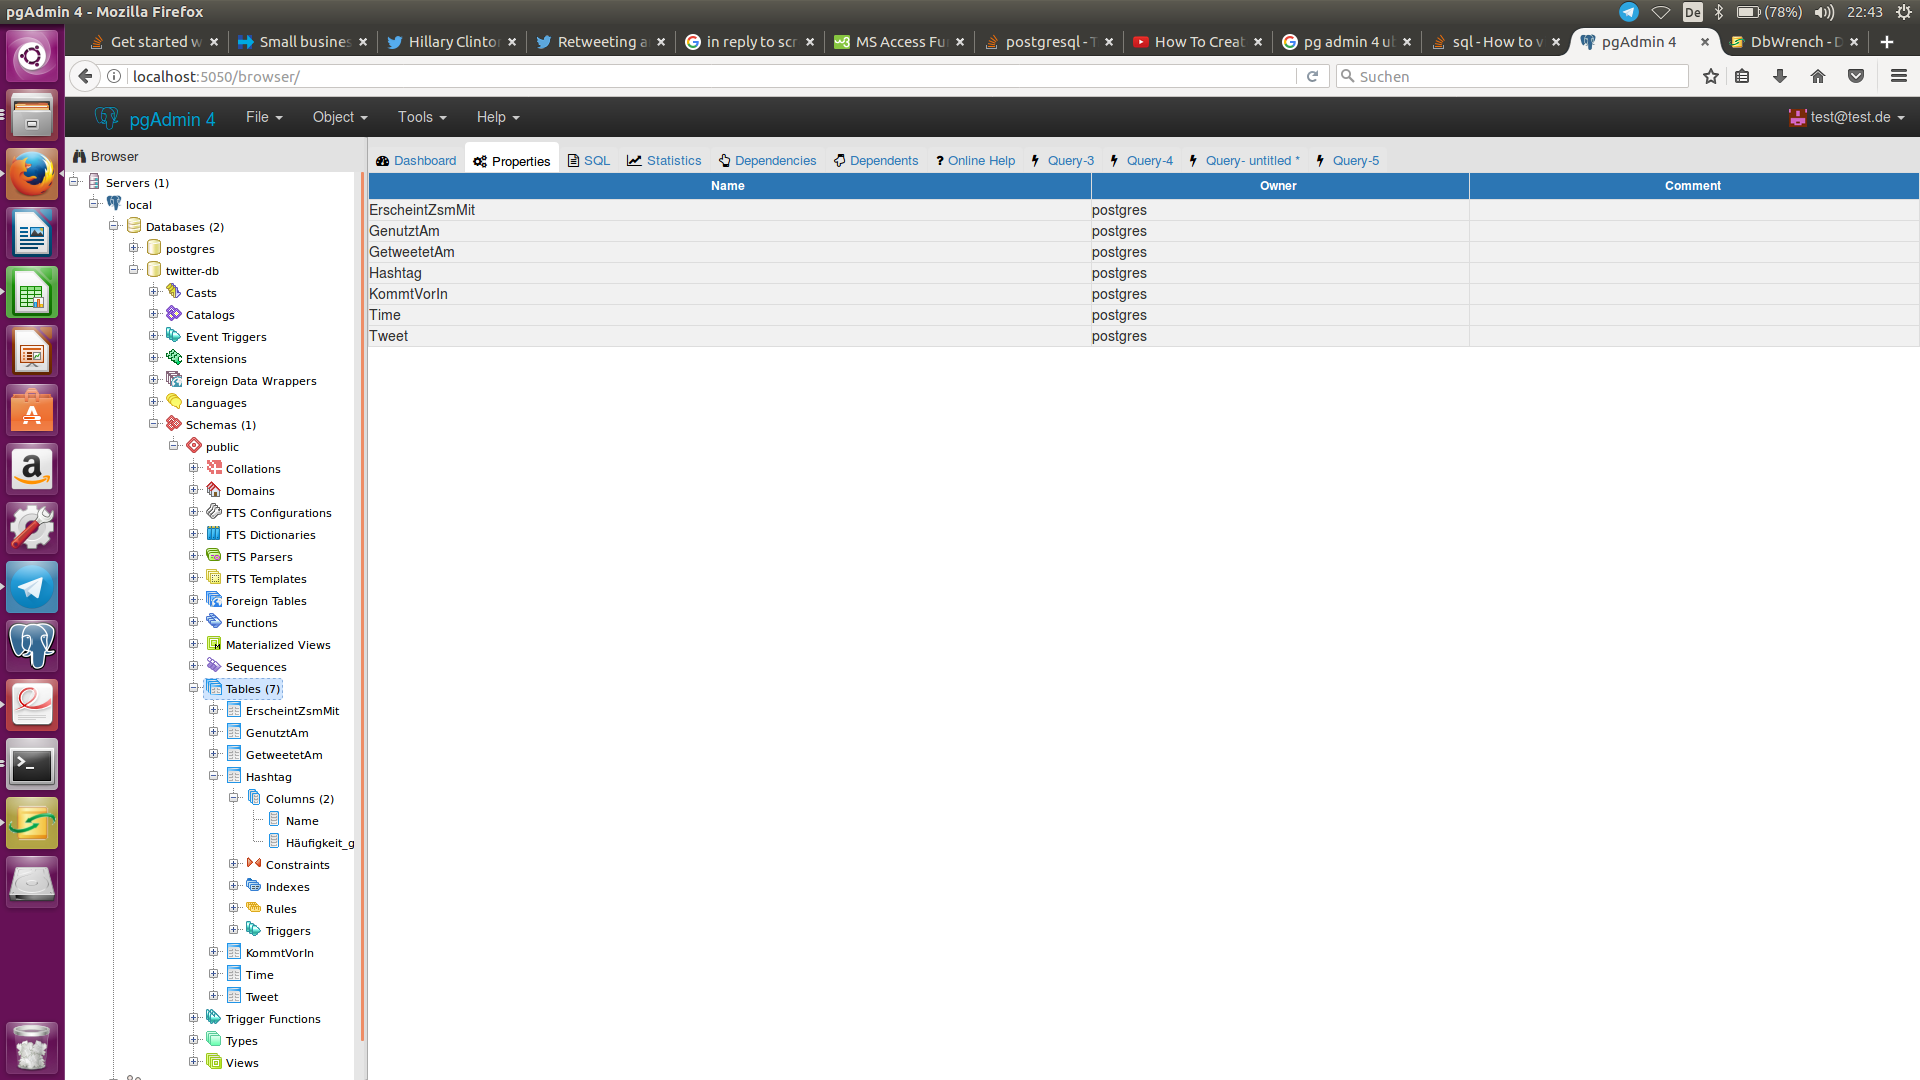
\includegraphics[width=12.0cm]{DatenbankErstellen2.png}}
\end{center}
Und hier noch eine Darstellung mit Dbwrench.
\begin{center}
  \makebox[\textwidth]{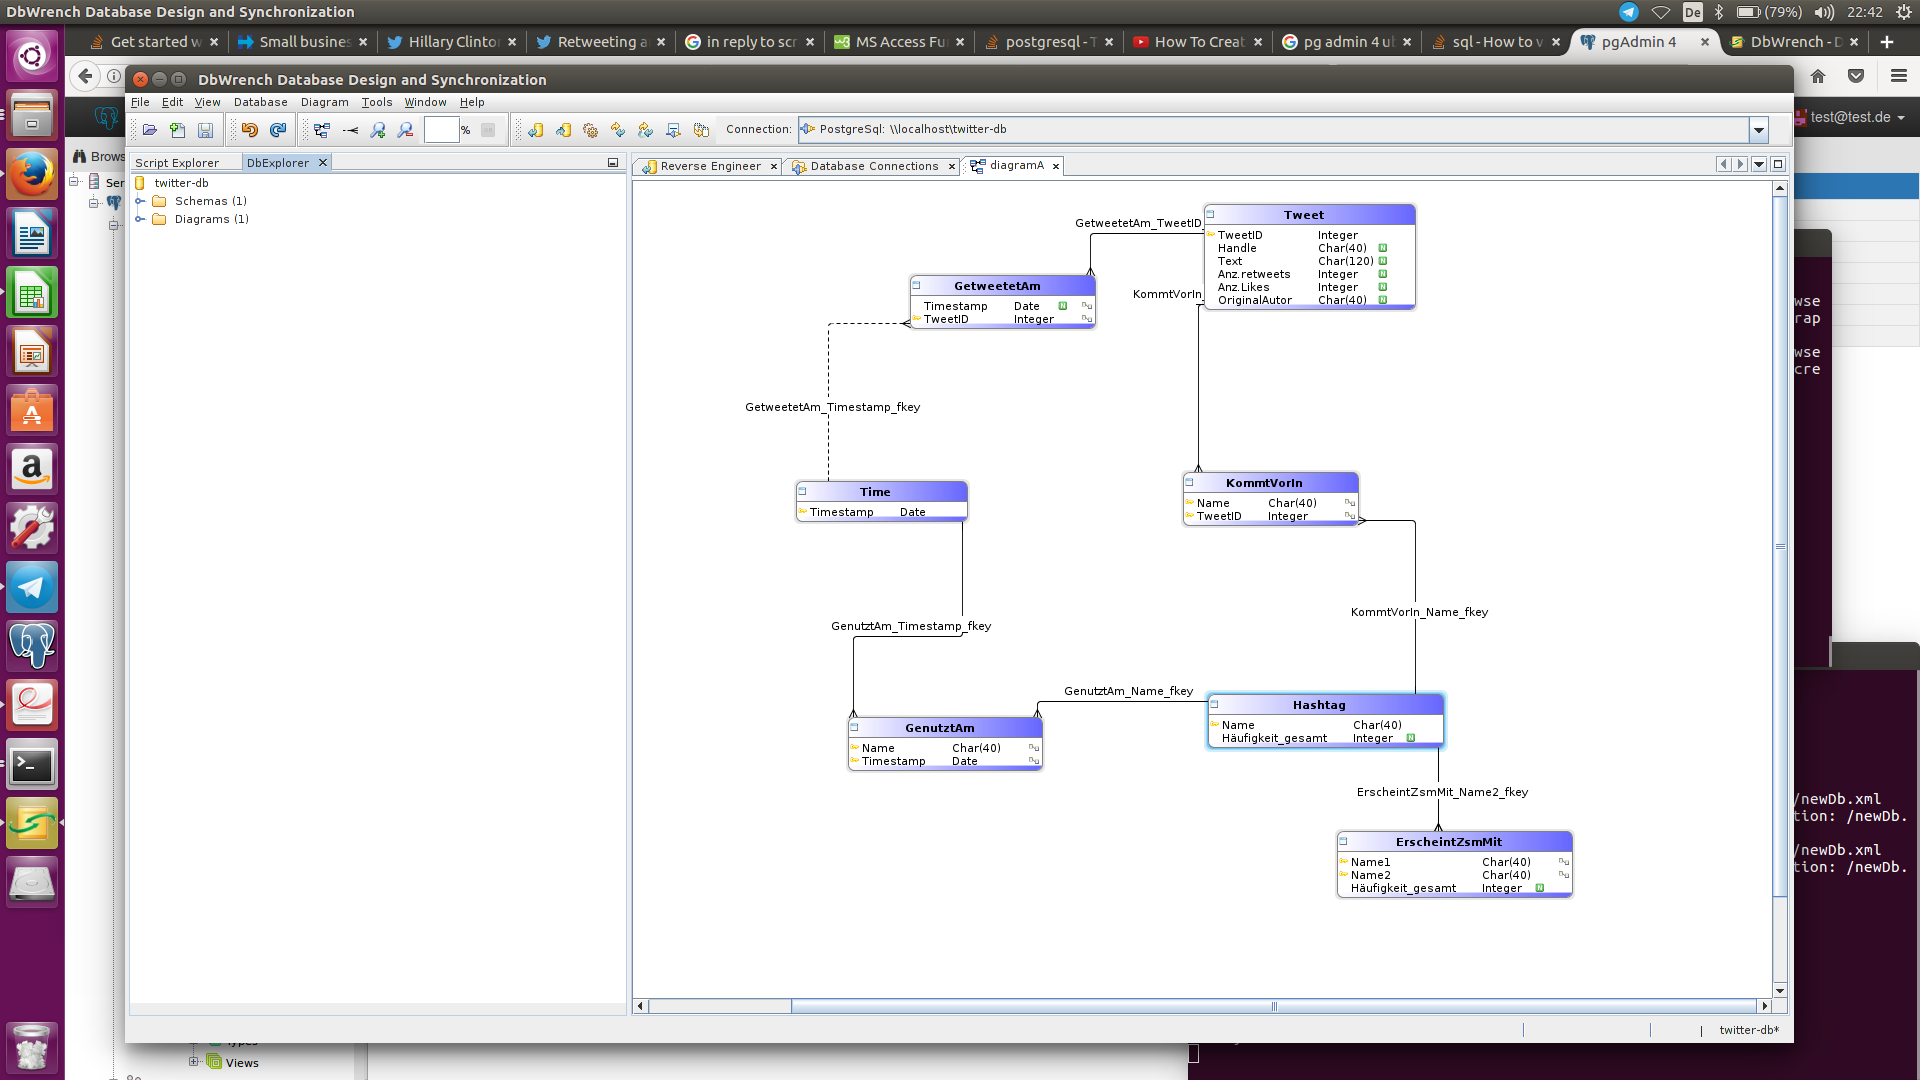
\includegraphics[width=12.0cm]{DatenbankErstellen1.png}}
\end{center}
\end{flushleft}

\newpage
\begin{flushleft}
\textbf{Schwierigkeiten}
\vspace{0.25cm}\\
Es war schwer ein ER-Modell zu finden welches Datenredundanz vermeidet. Zum Beispiel die richtige Position für das Datum und die Uhrzeit zu finden.\\
Wir waren uns auch nicht sicher ob der Datensatz bereits vollständig ist oder nicht, so dass wir erst überlegen mussten ob die Möglichkeit Neue Daten in die Datenbank einzufügen im er ER-Modell beachtet werden muss.\\
Und keiner von uns hat Twitter\\
\end{flushleft}

\end{document}
